\documentclass[
11pt% The default document font size, options: 10pt, 11pt, 12pt
%codirector, % Uncomment to add a codirector to the title page
]{charter} 

\usepackage{tikz}
\usepackage{float}
\usepackage{rotating}
\usetikzlibrary{fit,shapes.geometric,shapes, arrows.meta, arrows, positioning}



% El títulos de la memoria, se usa en la carátula y se puede usar el cualquier lugar del documento con el comando \ttitle
\titulo{Sistema de monitoreo de servicios de planta} 

% Nombre del posgrado, se usa en la carátula y se puede usar el cualquier lugar del documento con el comando \degreename
%\posgrado{Carrera de Especialización en Sistemas Embebidos} 
\posgrado{Carrera de Especialización en Internet de las Cosas} 
%\posgrado{Carrera de Especialización en Intelegencia Artificial}
%\posgrado{Maestría en Sistemas Embebidos} 
%\posgrado{Maestría en Internet de las cosas}

% Tu nombre, se puede usar el cualquier lugar del documento con el comando \authorname
\autor{Ing. Marcelo Roberto García} 

% El nombre del director y co-director, se puede usar el cualquier lugar del documento con el comando \supname y \cosupname y \pertesupname y \pertecosupname
\director{Mg. Ing. Gonzalo Nahuel Vaca}
\pertenenciaDirector{INVAP} 
% FIXME:NO IMPLEMENTADO EL CODIRECTOR ni su pertenencia
%\codirector{John Doe} % para que aparezca en la portada se debe descomentar la opción codirector en el documentclass
%\pertenenciaCoDirector{FIUBA}

% Nombre del cliente, quien va a aprobar los resultados del proyecto, se puede usar con el comando \clientename y \empclientename
\cliente{Ing. Guillermo Horacio Vidal}
\empresaCliente{ROEMMERS SAICF}

% Nombre y pertenencia de los jurados, se pueden usar el cualquier lugar del documento con el comando \jurunoname, \jurdosname y \jurtresname y \perteunoname, \pertedosname y \pertetresname.
\juradoUno{Nombre y Apellido (1)}
\pertenenciaJurUno{pertenencia (1)} 
\juradoDos{Nombre y Apellido (2)}
\pertenenciaJurDos{pertenencia (2)}
\juradoTres{Nombre y Apellido (3)}
\pertenenciaJurTres{pertenencia (3)}
 
\fechaINICIO{21 de junio de 2022}		%Fecha de inicio de la cursada de GdP \fechaInicioName
\fechaFINALPlan{9 de agosto de 2022} 	%Fecha de final de cursada de GdP
\fechaFINALTrabajo{22 de abril de 2023}	%Fecha de defensa pública del trabajo final


\begin{document}

\maketitle
\thispagestyle{empty}
\pagebreak


\thispagestyle{empty}
{\setlength{\parskip}{0pt}
\tableofcontents{}
}
\pagebreak


\section*{Registros de cambios}
\label{sec:registro}


\begin{table}[ht]
\label{tab:registro}
\centering
\begin{tabularx}{\linewidth}{@{}|c|X|c|@{}}
\hline
\rowcolor[HTML]{C0C0C0} 
Revisión & \multicolumn{1}{c|}{\cellcolor[HTML]{C0C0C0}Detalles de los cambios realizados} & Fecha      \\ \hline
0      & Creación del documento                                 &\fechaInicioName \\ \hline
1      & Se completa hasta el punto 5 inclusive                 & 5 de julio de 2022 \\ \hline
1.1      & Se corrigen errores de redacción y se modifican gráficos			               & 8 de julio de 2022 \\ \hline
2      & Se completa hasta el punto 9 inclusive 			               & 11 de julio de 2022 \\ \hline
2.1      & Se corrigen errores de redacción 			               & 14 de julio de 2022 \\ \hline
%		  Se puede agregar algo más \newline
%		  En distintas líneas \newline
%		  Así                                                    & dd/mm/aaaa \\ \hline
3      & Se completa hasta el punto 12 inclusive                & 25 de julio de 2022 \\ \hline
4      & Se completa el plan	                                 & 31 de julio de 2022\\ \hline

4.1      & Se corrigen errores de redacción                                 & 5 de agosto 2022\\ \hline
\end{tabularx}
\end{table}


\pagebreak



\section*{Acta de constitución del proyecto}
\label{sec:acta}

\begin{flushright}
Buenos Aires, \fechaInicioName
\end{flushright}

\vspace{2cm}

Por medio de la presente se acuerda con el  \authorname\hspace{1px} que su Trabajo Final de la \degreename\hspace{1px} se titulará ``\ttitle'', consistirá esencialmente en {la implementación de un servidor y una red de dispositivos distribuidos en planta para la lectura del estado de los servicios}, y tendrá un presupuesto preliminar estimado de {600} hs de trabajo y {USD 150}, con fecha de inicio \fechaInicioName\hspace{1px} y fecha de presentación pública \fechaFinalName.

Se adjunta a esta acta la planificación inicial.

\vfill

% Esta parte se construye sola con la información que hayan cargado en el preámbulo del documento y no debe modificarla
\begin{table}[ht]
\centering
\begin{tabular}{ccc}
\begin{tabular}[c]{@{}c@{}}Dr. Ing. Ariel Lutenberg \\ Director posgrado FIUBA\end{tabular} & \hspace{2cm} & \begin{tabular}[c]{@{}c@{}}\clientename \\ \empclientename \end{tabular} \vspace{2.5cm} \\ 
\multicolumn{3}{c}{\begin{tabular}[c]{@{}c@{}} \supname \\ Director del Trabajo Final\end{tabular}} \vspace{2.5cm} \\
%\begin{tabular}[c]{@{}c@{}}\jurunoname \\ Jurado del Trabajo Final\end{tabular}     &  & \begin{tabular}[c]{@{}c@{}}\jurdosname\\ Jurado del Trabajo Final\end{tabular}  \vspace{2.5cm}  \\
%\multicolumn{3}{c}{\begin{tabular}[c]{@{}c@{}} \jurtresname\\ Jurado del Trabajo Final\end{tabular}} \vspace{.5cm}                                                                     
\end{tabular}
\end{table}




\section{1. Descripción técnica-conceptual del proyecto a realizar}
\label{sec:descripcion}

%\begin{quote}


% El bloque "consigna" se usa para poner texto en rojo y dar una pequeña ayuda sobre cómo completar la sección
El proyecto a realizar es un sistema de monitoreo de servicios de planta. La empresa ROEMMERS elabora medicamentos en distintas presentaciones bajo las normas BPF (Buenas Prácticas de Fabricación), estas normas son exigidas por la A.N.M.A.T para autorizar su comercialización en el pais. %Ademas, en materia de reglamentación provincial, cumple con los requierimientos de OPDS y Acumar para el tratamiento de los efluentes industriales. 

Para el cumplimiento de las reglamentaciones y normas vigentes se cuenta con los siguientes sistemas de control:
\begin{itemize}
	\item Sistema de control HVAC (Heating and Ventilating Air Conditioned).
	\item Sistema de control de agua purificada, agua destilada y agua WFI (Water For Inyection).
	\item Sistema de control de vapor sanitario.
	\item Sistema de control de tratamiento de efluentes.
\end{itemize}
%A su vez, estos sistemas requieren la provisión de vapor, aire comprimido, agua potable, electricidad y gas natural. 

Los sistemas de control se operan mediante SCADAS, la operación es llevada a cabo por el departamento de mantenimiento de servicios, que también tiene como tarea asegurar los suministros de vapor, aire comprimido, agua potable, electricidad y gas natural para el funcionamiento de los sistemas.

Los SCADAS se encuentran distribuidos en dos salas de control denominadas DDC1 y DDC2. La conexión con los sistemas de control se realiza por medio de una red de fibra óptica (FO) compuesta por siete switches conectados en anillo. En la figura 1 se observa un diagrama conceptual de la red. 

En la actualidad, los suministros no se encuentran monitoreados mediante un SCADA, esto se debe a la distribución física de los servicios en la planta y a la escasa cantidad de variables que se requieren visualizar en comparación a los sistemas de control. Estas características vuelven inviable el despliegue de una red cableada y su hardware, motivo por el cual, la lectura del estado de los servicios se realiza in situ mediante la implementación de un calendario de revisiones diarias. Dichas revisiones son realizadas por los técnicos de mantenimiento de servicios.

En una tarea conjunta del departamento de mantenimiento de servicios y del departamento de mantenimiento electrónico, se propone la creación de un sistema de monitoreo de servicios de planta. El sistema utilizará la red de FO actual a la que se accederá con tecnología de tipo inalámbrica, esta tecnología permitirá reducir significativamente los costos de implementación.

En la figura 2 se observa el diagrama en bloques de una interfaz de conexión a la red, mientras que en la figura 3, se observa el diagrama en bloques de una interfaz de adquisición, ambas interfaces conforman el enlace entre la red y los puntos de servicio. 

Se espera que el proyecto agregue valor de la siguiente manera:
\begin{itemize}
	\item Optimizando el tiempo empleado en el relevamiento de los servicios.
	\item Aumentando la productividad del sector.
	\item Suministrando datos que aporten el desarrollo de estrategias de mantenimiento predictivo.
	\item Fomentando la iniciativa de ambos departamentos mediante equipos de trabajo.
\end{itemize}


%La planta cuenta con un departamento de mantenimiento que se encuentra formado por 3 sectores: mantenimiento mecánico, mantenimiento electrónico y mantenimiento de servcios. El deparatamento de mantenimiento de servicios opera los SCADAS mediante los cuales realiza la supervisión y control del funcionameinto de los sistemas de planta. Además, se encarga de garantizar la provisión de servicios requeridos por los sistemas de control.

%\vspace{25px}
\begin{figure}[htpb]
\centering 
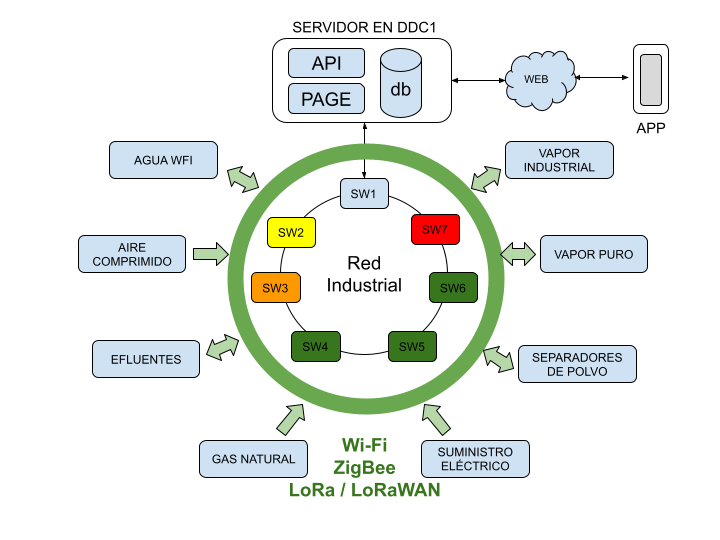
\includegraphics[width=0.75\textwidth]{./Figuras/diagrama_red_cel.png}
\caption{Diagrama de la red.}
\label{fig:diagBloques}
\end{figure}

\vspace{5px}
%\vspace{25px}

\begin{figure}[htpb]
\centering 
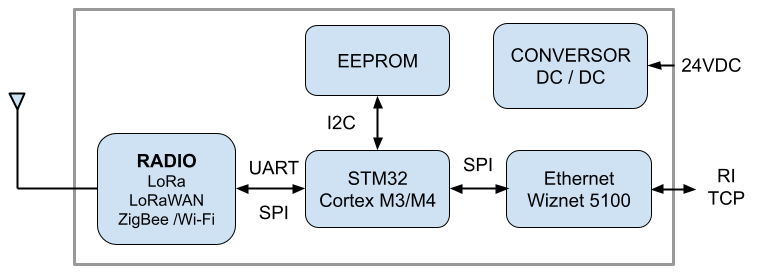
\includegraphics[width=.75\textwidth]{./Figuras/Interfaz_conn.png}
\caption{Diagrama en bloques de la interfaz de conexión.}
\label{fig:diagBloques}
\end{figure}

\vspace{5px}
%\vspace{25px}

\begin{figure}[htpb]
\centering 
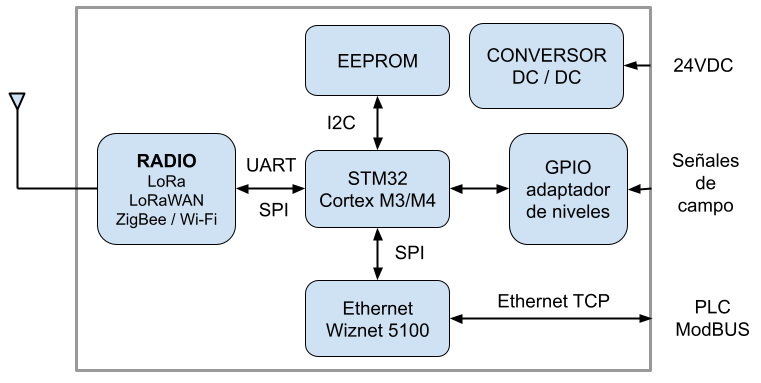
\includegraphics[width=.75\textwidth]{./Figuras/Interfaz_captura.png}
\caption{Diagrama en bloques de la interfaz de adquisición.}
\label{fig:diagBloques}
\end{figure}

\vspace{25px}

%\end{quote}






\section{2. Identificación y análisis de los interesados}
\label{sec:interesados}



\begin{table}[ht]
%\caption{Identificación de los interesados}
%\label{tab:interesados}
\begin{tabularx}{\linewidth}{@{}|l|X|X|l|@{}}
\hline
\rowcolor[HTML]{C0C0C0} 
Rol           & Nombre y Apellido & Organización 	& Puesto 	\\ \hline
%Auspiciante   &                   &              	&        	\\ \hline
Cliente       & \clientename      &\empclientename	& Jefe de Servicios
       	\\ \hline
%Impulsor      &                   &              	&        	\\ \hline
Responsable   & \authorname       & FIUBA        	& Alumno 	\\ \hline
%Colaboradores &                   &              	&        	\\ \hline
Orientador    & \supname	      & \pertesupname 	& Director Trabajo final \\ \hline
%Equipo        & miembro1 \newline 
				%&miembro2          &              	&        	\\ \hline
%Opositores    &                   &              	&        	\\ \hline
Usuario final &Supervisor y técnicos de manatenimiento de servicios                    &ROEMMERS SAICF              	&   -     	\\ \hline
\end{tabularx}
\end{table}

\begin{itemize}
	\item Cliente: cumple también el rol de usuario final.

\end{itemize}





\section{3. Propósito del proyecto}
\label{sec:proposito}




El propósito de este proyecto es desarrollar una solución tecnológica al sector de mantenimiento de servicios que permita optimizar sus tareas y brindar información para el registro y análisis de los datos de los sistemas. Además, incorporar el uso de nuevas tecnologías que permitan un rápido despliegue de la red.




%El propósito de este proyecto es:

%\begin{itemize}
%	\item Implementar la lectura de estado y variables críticas de los servicios utilizados para el %funcionamiento de los sistemas.
%	\item Incorporar el uso de nuevas tecnologías para el despliegue de red utilizando la red FO %actual.
%	\item Brindar herramientas al departamento de mantenimiento de servicios para poder implementar estategias de mantenimiento predictivo.
%	\item Reducir la frecuencia de chequeo in situ de las instalaciones.
%\end{itemize}


\section{4. Alcance del proyecto}
\label{sec:alcance}


El proyecto incluye en su alcance:
\begin{itemize} 
	\item Instalación de un servidor en sala de control DDC1.
	\item Diseño e instalación de las bases de datos.
	\item Desarrollo de una API (Application Programming Interface) para la comunicación con los dispositivos.
	\item Desarrollo de una SPA (Single Page Application) para el monitoreo de las variables.
	\item Desarrollo de una interfaz de conexión y una interfaz de adquisición capaces de transmitir información de manera inalámbrica utilizando los siguientes protocolos a evaluar: LoRa, LoRaWAN, Wi-Fi o Zigbee.
	
\end{itemize}

El proyecto no incluye en su alcance:
\begin{itemize}
	\item Conexión del sistema a Internet.
	\item Desarrollo de aplicación para teléfonos móviles.
\end{itemize}




\section{5. Supuestos del proyecto}
\label{sec:supuestos}


Para el desarrollo del presente proyecto se supone que:

\begin{itemize}
	\item Se tendrá acceso a un punto de servicio designado sobre el cual se realizará la instalación de la interfaz.
	\item Se dispondrá de recursos para la instalación de un servidor en la sala DDC1.
	\item Se tendrá acceso irrestricto al instrumental de laboratorio del departamento de mantenimiento electrónico.
	\item Se contará con la participación de un técnico del departamento de mantenimiento de servicios y de un técnico del departamento de mantenimiento electrónico durante el desarrollo del proyecto.
\end{itemize}



\section{6. Requerimientos}
\label{sec:requerimientos}

%\begin{consigna}{red}
\begin{enumerate}
	\item Requerimientos funcionales
		\begin{enumerate}
			\item La operación del sistema se debe realizar mediante un navegador de web.
			\item El sistema permitirá visualizar el estado de los servicios conectados.
			\item Las interfaces deben comunicarse entre si mediante tecnología LoRA, LoRaWAN, Zigbee o Wi-Fi.
			\item El sistema permitirá la visualización de alarmas de los servicios conectados.
			\item La interfaz debe conectarse a la red industrial cableada mediante un jack RJ-45.
			\item La interfaz de adquisición contará con entradas aisladas.
			\item Las interfaces contarán con indicadores visuales de alimentación, falla y conexión.
			\item El sistema permitirá visualizar el registro histórico de variables en intervalos configurables. 
			\item El sistema permitirá configurar usuarios y parámetros de conexión de los dispositivos de campo.
			\item El usuario podrá reiniciar la interfaz mediante un pulsador de reinicio.
		    \item Las interfaces contarán con un puerto para debugging/programming.
		    \item La alimentación de las interfaces debe ser de 24V DC/AC.
		    \item Las interfaces tendrán un gabinete que permita su montaje en pared con opción de montaje en riel DIN.
		\end{enumerate}

	\item Requerimientos de documentación
		\begin{enumerate}
			\item Se debe crear un manual de instalación del sistema.
			\item Se debe crear un manual de instalación de las interfaces.
			\item Se debe crear un manual de uso del sistema.
			\item Se debe crear un manual de uso de las interfaces.
			\item Se debe crear un protocolo de pruebas para validar el funcionamiento del sistema.
			\item Se debe generar un informe con las pruebas de funcionamiento del sistema en campo.
			\item Se debe generar un informe de avance del proyecto.
			\item Se debe generar una memoria del proyecto.

		\end{enumerate}
	%\item Requerimiento de testing...
	%\item Requerimientos de la interfaz...
	%\item Requerimientos interoperabilidad...
	%\item etc...
\end{enumerate}

%Leyendo los requerimientos se debe poder interpretar cómo será el proyecto y su funcionalidad.

%Indicar claramente cuál es la prioridad entre los distintos requerimientos y si hay requerimientos opcionales. 

%No olvidarse de que los requerimientos incluyen a las regulaciones y normas vigentes!!!

%Y al escribirlos seguir las siguientes reglas:
%\begin{itemize}
%	\item Ser breve y conciso (nadie lee cosas largas). 
%	\item Expresar los requerimientos en términos que sean cuantificables y medibles.
%\end{itemize}

%\end{consigna}

\section{7. Historias de usuarios (\textit{Product backlog})}
\label{sec:backlog}


%Descripción: En esta sección se deben incluir las historias de usuarios y su ponderación (\textit{history points}). Recordar que las historias de usuarios son descripciones cortas y simples de una característica contada desde la perspectiva de la persona que desea la nueva capacidad, generalmente un usuario o cliente del sistema. La ponderación es un número entero que representa el tamaño de la historia comparada con otras historias de similar tipo.

Las historias de usuarios se clasifican numéricamente de acuerdo al grado de complejidad de su implementación, a continuación se detallan dichos valores:

\begin{itemize}
	\item 1 punto: la historia demanda un desafío básico, no requiere del uso de tecnologías adicionales.
	\item 2 puntos: la historia demanda conocimientos de una tecnología.
	\item 4 puntos: la historia demanda conocimientos de múltiples tecnologías.
	\item 8 puntos: la historia demanda conocimientos avanzados de múltiples tecnologías.
	\item 16 puntos: la historia demanda conocimientos avanzados de múltiples tecnologías y del hardware instalado.
\end{itemize}

A continuación se detallan las historias de usuario:

\begin{itemize}
	\item Historia 1 
\begin{itemize}
	\item Como jefe de mantenimiento de servicios quiero poder verificar el estado general de los sistemas para saber si se encuentran operativos. 
	\item\textit{Story points: \textbf{4}}, la historia requiere del uso de tecnologías web, networking y conocimiento del protocolo ModBUS.
\end{itemize}
	\item Historia 2
\begin{itemize}
	\item Como supervisor de servicios quiero poder visualizar las alarmas de los sistemas para determinar una intervención inmediata.
	\item \textit{Story points: \textbf{8}}, la historia requiere del uso de tecnologías web, networking, gestión de base de datos básica y conocimiento del hardware utilizado.
\end{itemize}
	\item Historia 3
\begin{itemize}
	\item Como técnico de mantenimiento quiero poder visualizar las alarmas y variables históricas de los sistemas para poder asistir su mantenimiento.
	\item \textit{Story points: \textbf{8}}, la historia requiere del uso de tecnologías web, networking, gestión de base de datos avanzada y conocimiento del hardware utilizado.
\end{itemize}
	\item Historia 4
\begin{itemize}
	\item Como técnico de mantenimiento electrónico necesito acceder a todos los componentes del sistema para verificar su funcionamiento.
	\item \textit{Story points: \textbf{16}}, la historia requiere del uso de tecnologías web, networking, gestión de base de datos avanzada y conocimiento avanzado del hardware utilizado.
\end{itemize}
	\item Historia 5
\begin{itemize}
	\item Como miembro de seguridad de planta quiero saber si existe algún problema para reportarlo al responsable del sector.
	\item \textit{Story points: \textbf{1}}, la historia requiere una instalación cableada básica.
\end{itemize}

\end{itemize}
%El formato propuesto es: "como [rol] quiero [tal cosa] para [tal otra cosa]."

%Se debe indicar explícitamente el criterio para calcular los \textit{story points} de cada historia


\section{8. Entregables principales del proyecto}
\label{sec:entregables}

Los entregables del proyecto son:

\begin{itemize}
	\item Backend y frontend operativo en servidor de la red industrial.
	\item Prototipos de ambas interfaces en funcionamiento.
	\item Planos eléctricos de conexión de ambas interfaces.
	\item Diagrama de red de la instalación.
	\item Informe de la instalación con la configuración de las interfaces y las variables del proceso.
	\item Manual de uso y configuración del sistema.
	\item Manual de uso, configuración e instalación de las interfaces.
		
\end{itemize}


\section{9. Desglose del trabajo en tareas}
\label{sec:wbs}


\begin{enumerate}
\item Planificación (15 hs)
	\begin{enumerate}
	\item Análisis de la problemática actual (8 hs).
	\item Definición del servicio de planta con el que se va a trabajar (1 hs).
	\item Análisis y definición de datos a extraer del servicio (2 hs).
	\item Nombramiento de los técnicos que participarán en las tareas del proyecto (1 hs).
	\item Gestión del calendario de intervenciones en el servicio (3 hs).
	\end{enumerate}
\item Investigación (62 hs)
	\begin{enumerate}
	\item Prueba en campo de tecnologías LoRA / LoRAWAN (24 hs).
	\item Prueba en campo de tecnologías Zigbee / Wi-Fi (24 hs).
	\item Determinar método de medición de datos (2 hs).
	\item Evaluar herramientas de representación de datos con dashboards y gráficos (12 hs).
	\end{enumerate}
\item Backend (63 hs)
	\begin{enumerate}
	\item Instalación del servidor Linux (3 hs).
	\item Diseño e instalación de la base de datos (15 hs).
	\item Creación de la API (40 hs).
	\end{enumerate}
\item Frontend (75 hs)
	\begin{enumerate}
	\item Creación de la SPA (38 hs).
	\item Integración de las herramientas para la representación de datos (32 hs).
	\item Integración con backend (6 hs).
	\end{enumerate}
\item Interfaz de comunicación (146 hs)
	\begin{enumerate}
	\item Desarrollo del firmware de la interfaz de comunicación (40 hs).
	\item Creación de biblioteca ModBUS (18 hs).
	\item Creación de biblioteca SPI para modulo Ethernet W5100 (35 hs).
	\item Creación de biblioteca para radio del dispositivo (25 hs).
	\item Diseño del circuito impreso de la interfaz de comunicación (12 hs).
	\item Armado y prueba del circuito impreso en laboratorio (8 hs).
	\item Diseño del gabinete (8 hs).
	\end{enumerate}
\item Interfaz de adquisición (88 hs)
	\begin{enumerate}
	\item Desarrollo del firmware de la interfaz de adquisición (35 hs).
	\item Diseño del circuito GPIO adaptador de niveles (12 hs).
	\item Prueba del circuito en laboratorio (4 hs).
	\item Diseño del circuito impreso de la interfaz de adquisición (18 hs).
	\item Armado y prueba del circuito impreso de la interfaz de adquisición (8 hs).
	\item Diseño del gabinete (11 hs).
	\end{enumerate}
\item Pruebas del sistema (64 hs)
	\begin{enumerate}
	\item Creación y ejecución del protocolo de pruebas del sistema (25 hs)
	\item Seguimiento del funcionamiento del sistema en campo (39 hs).
	\end{enumerate}
\item Cierre (91 hs)
	\begin{enumerate}
	\item Creación de manuales de uso e instalación (18 hs).
	\item Creación de informes de avance de proyecto (15 hs).
	\item Creación de informe final de desempeño del proyecto (20 hs).
	\item Creación de la memoria del trabajo (29 hs).
	\item Creación del video de demostración (8 hs).
	\item Defensa pública y agradecimientos(1 hs).
	\end{enumerate}
\end{enumerate}

Cantidad total de horas: (600 hs)

\section{10. Diagrama de Activity On Node}
\label{sec:AoN}



EL diagrama de Activity On Node representa la dependencia entre las tareas listadas en la sección 9. Las tareas se agrupan por categorías: planificación, investigación, backend, frontend, interfaz de comunicación, interfaz de adquisición, pruebas del sistema y cierre.

El tiempo empleado para ejecutar cada tarea se representa mediante la variable \textit{"T"}, cuya unidad es cantidad de horas. Además, las tareas se agrupan en categorías identificadas mediante colores los cuales se detallan en el cuadro de referencias de la figura 4.

Finalmente se obtiene el camino crítico del diagrama de Activity On Node.

\begin{table}[ht]
\begin{tabularx}{\linewidth}{@{}|l|X|l|@{}}
\hline
\rowcolor[HTML]{C0C0C0} 
Descripción           & Tareas & T \\ \hline	%& Puesto 	\\ \hline
%Auspiciante   &                   &              	&        	\\ \hline
Camino crítico      & 1.1 - 1.5 - 2.1 - 2.4 - 4.1 - 4.2 - 4.3 - 5.1 - 5.2 - 5.3 - 6.1 - 7.2 - 8.2 - 8.3 - 8.4 - 8.5 - 8.6      &364	%& Jefe de Servicios
       	\\ \hline
%Impulsor      &                   &              	&        	\\ \hline
%Responsable   & \authorname       & FIUBA        	& Alumno 	\\ \hline
%Colaboradores &                   &              	&        	\\ \hline
%Orientador    & \supname	      & \pertesupname 	& Director Trabajo final \\ \hline
%Equipo        & miembro1 \newline 
				%&miembro2          &              	&        	\\ \hline
%Opositores    &                   &              	&        	\\ \hline
%Usuario final &Supervisor y técnicos de manatenimiento de servicios                    &ROEMMERS SAICF              	&   -     	\\ \hline
\end{tabularx}
\end{table}



%La figura \ref{fig:AoN} fue elaborada con el paquete latex tikz y pueden consultar la siguiente referencia \textit{online}:

%\url{https://www.overleaf.com/learn/latex/LaTeX_Graphics_using_TikZ:_A_Tutorial_for_Beginners_(Part_3)\%E2\%80\%94Creating_Flowcharts}


\begin{figure}[htpb]
%\centering 
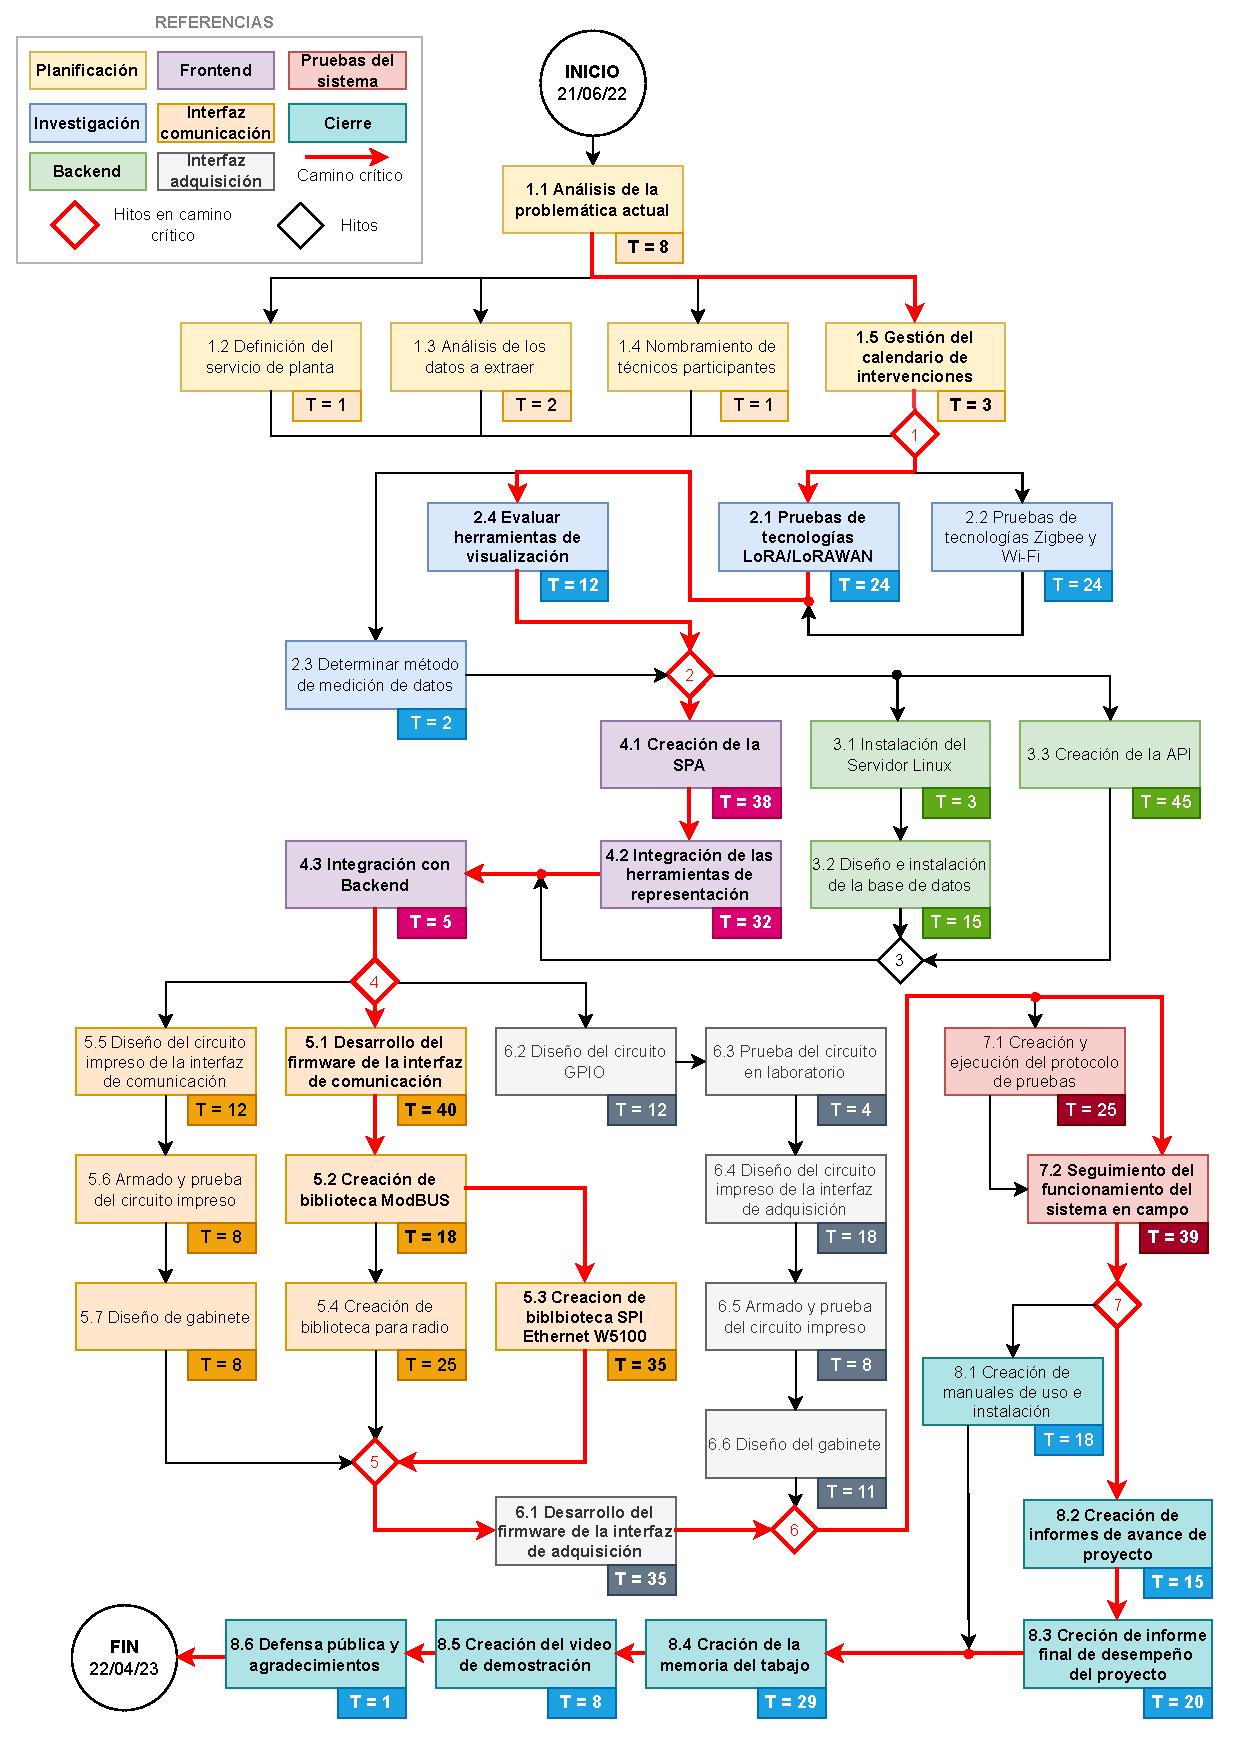
\includegraphics[width=1\textwidth]{./Figuras/aonv8.drawio.pdf}
\caption{Diagrama en  \textit{Activity on Node.}}
\label{fig:diagBloques}
\end{figure}

%\begin{figure}[htpb]
%\centering 
%\includegraphics[width=.8\textwidth]{./Figuras/AoN.png}
%\caption{Diagrama en \textit{Activity on Node}}
%\label{fig:AoN}
%\end{figure}

%Indicar claramente en qué unidades están expresados los tiempos.
%De ser necesario indicar los caminos semicríticos y analizar sus tiempos mediante un cuadro.
%Es recomendable usar colores y un cuadro indicativo describiendo qué representa cada color, %como se muestra en el siguiente ejemplo:


%\begin{landscape}
\section{11. Diagrama de Gantt}
\label{sec:gantt}

A partir de los diagramas de \emph{Activity On Node} de la sección \ref{sec:AoN} se realizó un diagrama de Gantt.\\

%\begin{table}[]
%\begin{tabular}{lll}
%\rowcolor[HTML]{C0C0C0} 
 % &\textbf{inicio}& \textbf{fin}  \\
 %\footnotesize{\textbf{1}-Planificacion }&\footnotesize{21/07/2022}  &\footnotesize{27/07/2022}  \\
 %\footnotesize{1.1 Análisis de la problemática actual}&\footnotesize{21/07/2022}&\footnotesize{27/07/2022}\\
 %\footnotesize{1.2 Definición del servicio de planta con el que se va a trabajar}&\footnotesize{21/07/2022}&\footnotesize{27/07/2022}\\
 %\footnotesize{1.3 Análisis y definición de datos a extraer del servicio}&\footnotesize{21/07/2022}&\footnotesize{27/07/2022}\\
 %\footnotesize{1.4 Nombramiento de los técnicos que participarán en las tareas del proyecto}&\footnotesize{21/07/2022}&\footnotesize{27/07/2022}\\
 %\footnotesize{1.5 Gestión del calendario de intervenciones en el servicio}&\footnotesize{21/07/2022}&\footnotesize{27/07/2022}\\
 %\footnotesize{\textit {Hito 1 Finalización de la planificación}}&\footnotesize{21/07/2022}&\footnotesize{27/07/2022}\\
 %\rowcolor[HTML]{C0C0C0} 
 %\footnotesize{2 Investigación}&\footnotesize{21/07/2022}&\footnotesize{27/07/2022}\\
 %\footnotesize{2.1 Prueba en campo de tecnologías LoRA / LoRAWAN}&\footnotesize{21/07/2022}&\footnotesize{27/07/2022}\\
 %\footnotesize{2.2 Prueba en campo de tecnologías Zigbee / Wi-Fi}&\footnotesize{21/07/2022}&\footnotesize{27/07/2022}\\
 %\footnotesize{2.3 Determinar método de medición de datos}&\footnotesize{21/07/2022}&\footnotesize{27/07/2022}\\
 %\footnotesize{2.4 Evaluar herramientas de representación de datos con dashboards y gráficos}&\footnotesize{21/07/2022}&\footnotesize{27/07/2022}\\
 %\footnotesize{\textit {Hito 2 Investigación de tecnologías realizada}}&\footnotesize{21/07/2022}&\footnotesize{27/07/2022}\\
 %\rowcolor[HTML]{C0C0C0}
 %\footnotesize{3 Backend}&\footnotesize{21/07/2022}&\footnotesize{27/07/2022}\\
 %\footnotesize{3.1 Instalación del servidor Linux}&\footnotesize{21/07/2022}&\footnotesize{27/07/2022}\\
 %\footnotesize{3.2 Diseño e instalación de la base de datos}&\footnotesize{21/07/2022}&\footnotesize{27/07/2022}\\
 %\footnotesize{3.3 Creación de la API}&\footnotesize{21/07/2022}&\footnotesize{27/07/2022}\\
 %\footnotesize{\textit {Hito 3 Finalización del Backend}}&\footnotesize{21/07/2022}&\footnotesize{27/07/2022}\\
 %\rowcolor[HTML]{C0C0C0}
 %\footnotesize{4 Frontend}&\footnotesize{21/07/2022}&\footnotesize{27/07/2022}\\
 %\footnotesize{4.1 Creación de la SPA}&\footnotesize{21/07/2022}&\footnotesize{27/07/2022}\\
 %\footnotesize{4.2 ntegración de las herramientas para la representación de datos}&\footnotesize{21/07/2022}&\footnotesize{27/07/2022}\\
 %\footnotesize{4.3 Integración con backend}&\footnotesize{21/07/2022}&\footnotesize{27/07/2022}\\
 %\footnotesize{\textit {Hito 4 Finalización del Frontend}}&\footnotesize{21/07/2022}&\footnotesize{27/07/2022}\\
 %\rowcolor[HTML]{C0C0C0}
 %\footnotesize{5 Interfaz de comunicación}&\footnotesize{21/07/2022}&\footnotesize{27/07/2022}\\
 %\footnotesize{5.1 Desarrollo del firmware de la interfaz de comunicación}&\footnotesize{21/07/2022}&\footnotesize{27/07/2022}\\
 %\footnotesize{5.2 Creación de biblioteca ModBUS}&\footnotesize{21/07/2022}&\footnotesize{27/07/2022}\\
 %\footnotesize{5.3 Creación de biblioteca SPI para modulo Ethernet W5100}&\footnotesize{21/07/2022}&\footnotesize{27/07/2022}\\
 %\footnotesize{5.4 Creación de biblioteca para radio del dispositivo}&\footnotesize{21/07/2022}&\footnotesize{27/07/2022}\\
 %\footnotesize{5.5 Diseño del circuito impreso de la interfaz de comunicación}&\footnotesize{21/07/2022}&\footnotesize{27/07/2022}\\
 %\footnotesize{5.6 Armado y prueba del circuito impreso en laboratorio}&\footnotesize{21/07/2022}&\footnotesize{27/07/2022}\\
 %\footnotesize{5.7 Diseño del gabinete}&\footnotesize{21/07/2022}&\footnotesize{27/07/2022}\\
 %\footnotesize{\textit {Hito 5 Interfaz de comunicación finalizada}}&\footnotesize{21/07/2022}&\footnotesize{27/07/2022}\\
 %\rowcolor[HTML]{C0C0C0}
 %\footnotesize{6 Interfaz de adquisición}&\footnotesize{21/07/2022}&\footnotesize{27/07/2022}\\
 %\footnotesize{6.1 Desarrollo del firmware de la interfaz de adquisición}&\footnotesize{21/07/2022}&\footnotesize{27/07/2022}\\
 %\footnotesize{6.2 Diseño del circuito GPIO adaptador de niveles}&\footnotesize{21/07/2022}&\footnotesize{27/07/2022}\\
 %\footnotesize{6.3 Prueba del circuito en laboratorio}&\footnotesize{21/07/2022}&\footnotesize{27/07/2022}\\
 %\footnotesize{6.4 Diseño del circuito impreso de la interfaz de adquisición}&\footnotesize{21/07/2022}&\footnotesize{27/07/2022}\\
 %\footnotesize{6.5 Armado y prueba del circuito impreso de la interfaz de adquisición}&\footnotesize{21/07/2022}&\footnotesize{27/07/2022}\\
 %\footnotesize{6.6 Diseño del gabinete}&\footnotesize{21/07/2022}&\footnotesize{27/07/2022}\\
 %\footnotesize{\textit {Hito 6 Desarrollo del hardware finalizado}}&\footnotesize{21/07/2022}&\footnotesize{27/07/2022}\\
 %\rowcolor[HTML]{C0C0C0}
 %\footnotesize{7 Pruebas del sistema}&\footnotesize{21/07/2022}&\footnotesize{27/07/2022}\\
 %\footnotesize{7.1 Creación y ejecución del protocolo de pruebas del sistema }&\footnotesize{21/07/2022}&\footnotesize{27/07/2022}\\
 %\footnotesize{7.2 Seguimiento del funcionamiento del sistema en campo}&\footnotesize{21/07/2022}&\footnotesize{27/07/2022}\\
 %\footnotesize{\textit {Hito 7 Pruebas de funcionamiento y evaluación finalizadas}}&\footnotesize{21/07/2022}&\footnotesize{27/07/2022}\\
 %\rowcolor[HTML]{C0C0C0}
 %\footnotesize{8 Cierre}&\footnotesize{21/07/2022}&\footnotesize{27/07/2022}\\
 %\footnotesize{8.1 Creación de manuales de uso e instalación}&\footnotesize{21/07/2022}&\footnotesize{27/07/2022}\\
 %\footnotesize{8.2 Creación de informes de avance de proyecto}&\footnotesize{21/07/2022}&\footnotesize{27/07/2022}\\\
 %\footnotesize{8.3 Creación de informe final de desempeño del proyecto}&\footnotesize{21/07/2022}&\footnotesize{27/07/2022}\\
 %\footnotesize{8.4 Creación de la memoria del trabajo}&\footnotesize{21/07/2022}&\footnotesize{27/07/2022}\\
 %\footnotesize{8.5 Creación del video de demostración}&\footnotesize{21/07/2022}&\footnotesize{27/07/2022}\\
 %\footnotesize{8.6 Defensa pública y agradecimientos}&\footnotesize{21/07/2022}&\footnotesize{27/07/2022}\\
 %\footnotesize{\textit {Hito 8 Fin del proyecto}}&\footnotesize{21/07/2022}&\footnotesize{27/07/2022}\\
% &  &  \\
% &  & 
%\end{tabular}
%\caption{Tabla de \textit{Gantt.}}
%\end{table}


\begin{figure}[H]
\centering

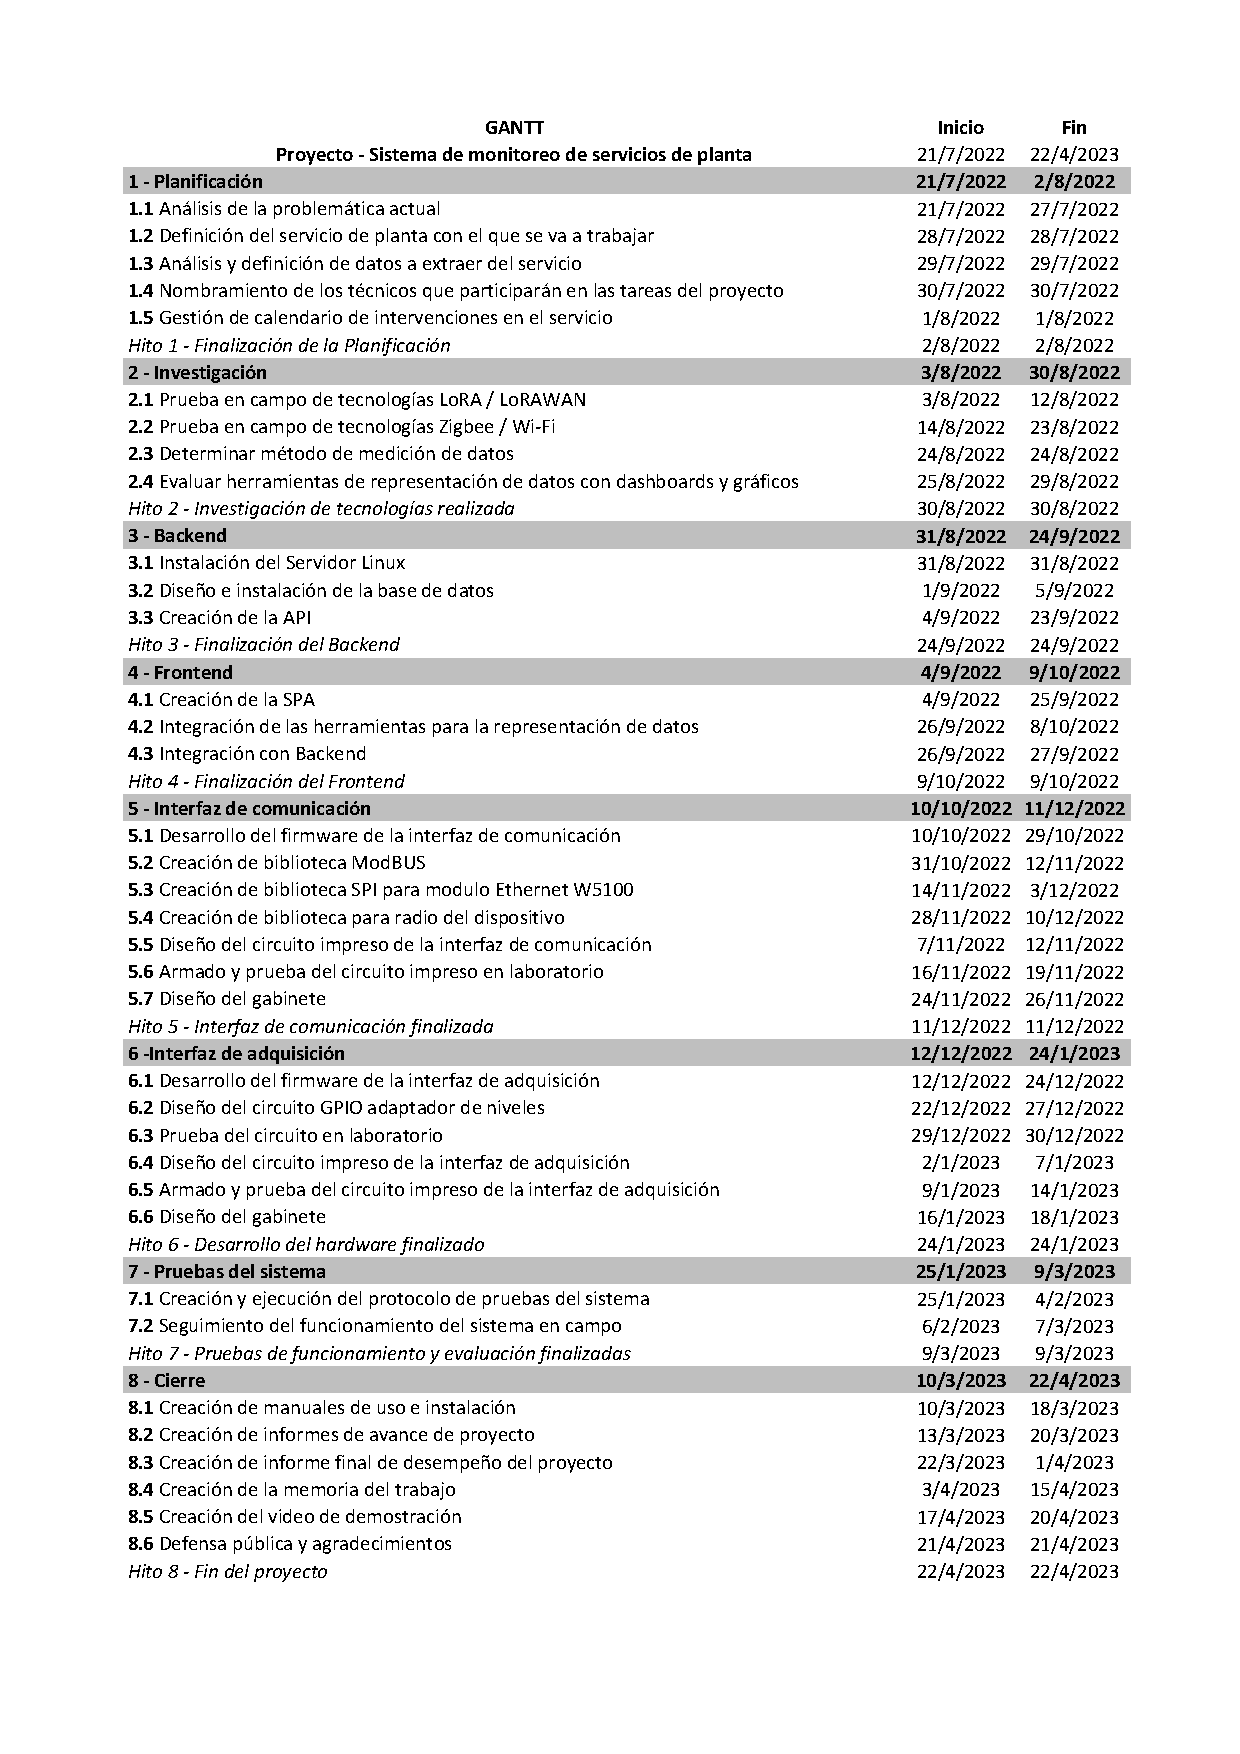
\includegraphics[width=0.88\textwidth]{./Figuras/tablagantt.pdf}

\caption{Tabla de \textit{Gantt.}}
\label{fig:gantt1}
\end{figure}

\begin{figure}[htpb]
\centering
%\begin{sidewaysfigure}[htpb]
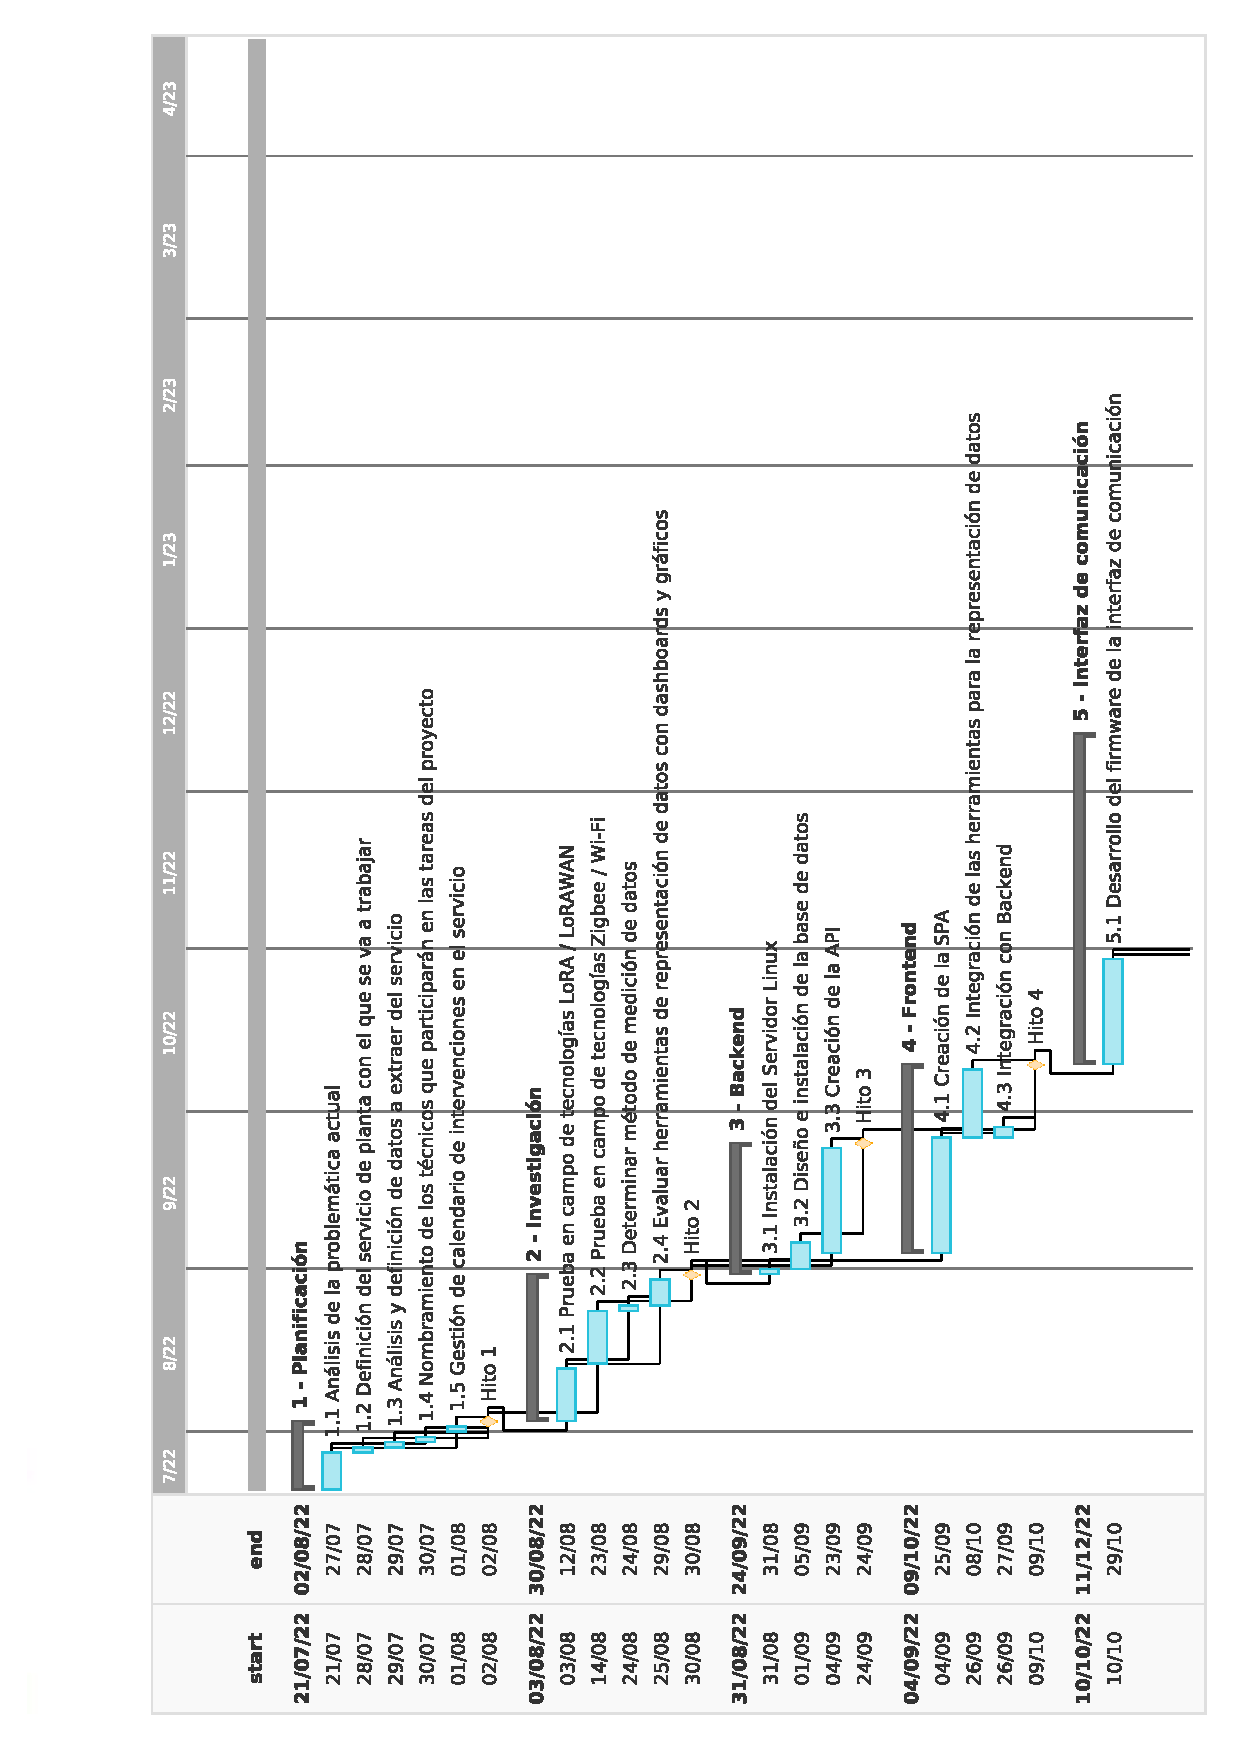
\includegraphics[width=1\textwidth]{./Figuras/gantt_A5_1_ed2.pdf}
\caption{Diagrama de \textit{Gantt parte 1.}}
\label{fig:gantt2}
\end{figure}

%\end{figure}

%\end{landscape}
%\begin{landscape}
%\begin{sidewaysfigure}[htpb]


\begin{figure}[htpb]
\centering 
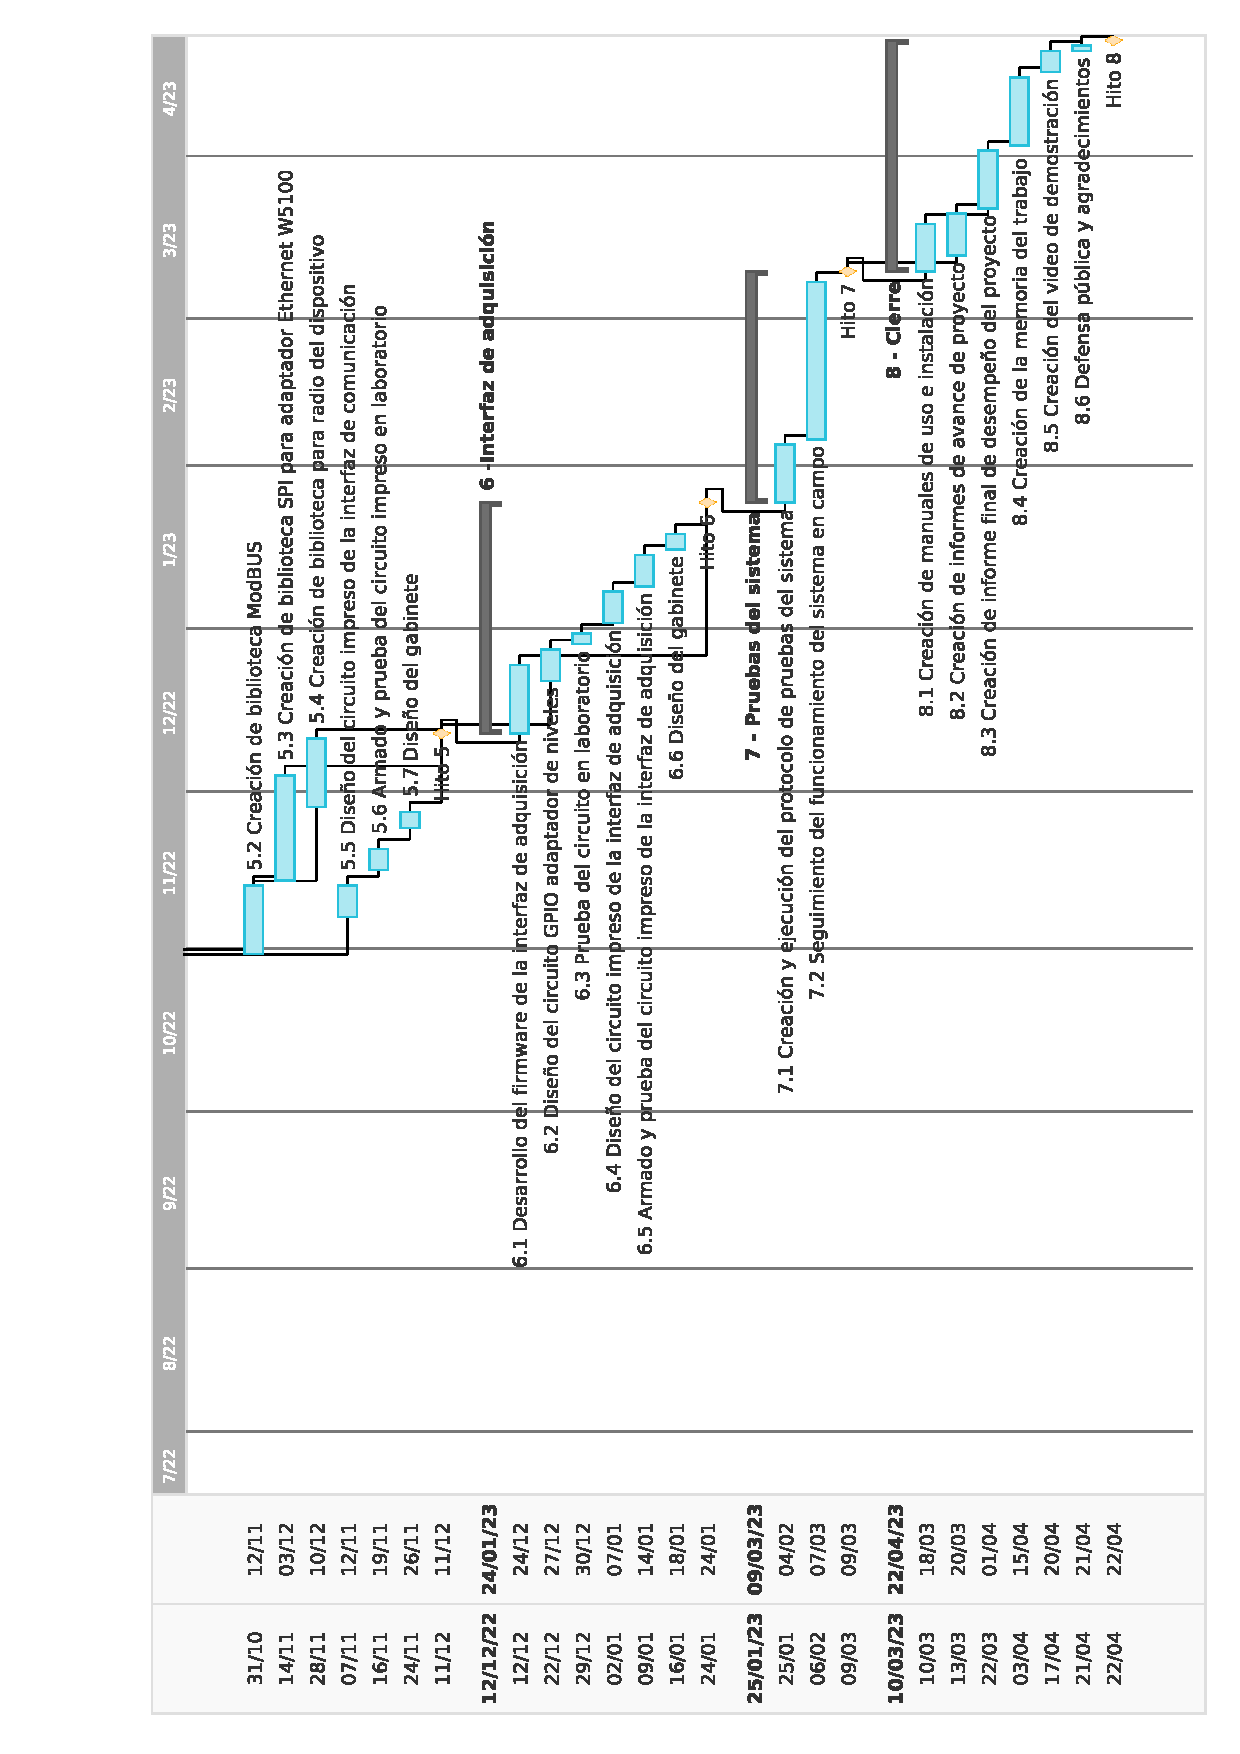
\includegraphics[width=1\textwidth]{./Figuras/gantt_A5_2_ed2.pdf}
\caption{Diagrama en \textit{Gantt parte 2.}}
\label{fig:gantt3}
%\end{sidewaysfigure}
\end{figure}


%\end{figure}
%Existen muchos programas y recursos \textit{online} para hacer diagramas de gantt, entre los cuales destacamos:

%\begin{itemize}
%\item Planner
%\item GanttProject
%\item Trello + \textit{plugins}. En el siguiente link hay un tutorial oficial: \\ \url{https://blog.trello.com/es/diagrama-de-gantt-de-un-proyecto}
%\item Creately, herramienta online colaborativa. \\\url{https://creately.com/diagram/example/ieb3p3ml/LaTeX}
%\item Se puede hacer en latex con el paquete \textit{pgfgantt}\\ \url{http://ctan.dcc.uchile.cl/graphics/pgf/contrib/pgfgantt/pgfgantt.pdf}
%\end{itemize}

%Pegar acá una captura de pantalla del diagrama de Gantt, cuidando que la letra sea suficientemente grande como para ser legible. 
%Si el diagrama queda demasiado ancho, se puede pegar primero la ``tabla'' del Gantt y luego pegar la parte del diagrama de barras del diagrama de Gantt.

%Configurar el software para que en la parte de la tabla muestre los códigos del EDT (WBS).\\
%Configurar el software para que al lado de cada barra muestre el nombre de cada tarea.\\
%Revisar que la fecha de finalización coincida con lo indicado en el Acta Constitutiva.

%En la figura \ref{fig:gantt}, se muestra un ejemplo de diagrama de gantt realizado con el paquete de \textit{pgfgantt}. En la plantilla pueden ver el código que lo genera y usarlo de base para construir el propio.

%\begin{figure}[htbp]
%\begin{center}
%\begin{ganttchart}{1}{12}
%  \gantttitle{2020}{12} \\
%  \gantttitlelist{1,...,12}{1} \\
%  \ganttgroup{Group 1}{1}{7} \\
%  \ganttbar{Task 1}{1}{2} \\
%  \ganttlinkedbar{Task 2}{3}{7} \ganttnewline
%  \ganttmilestone{Milestone o hito}{7} \ganttnewline
%   \ganttbar{Final Task}{8}{12}
%  \ganttlink{elem2}{elem3}
%  \ganttlink{elem3}{elem4}
%\end{ganttchart}
%\end{center}
%\caption{Diagrama de gantt de ejemplo}
%\label{fig:gantt}
%\end{figure}


%\begin{landscape}
%\begin{figure}[htpb]
%\centering 
%\includegraphics[height=.85\textheight]{./Figuras/Gantt-2.png}
%\caption{Ejemplo de diagrama de Gantt rotado}
%\label{fig:diagGantt}
%\end{figure}

%\end{landscape}


\flushleft

\section{12. Presupuesto detallado del proyecto}
\label{sec:presupuesto}


A continuación se detallan los costos del proyecto.



\begin{table}[htpb]
\centering
\begin{tabularx}{\linewidth}{@{}|X|c|r|r|@{}}
\hline
\rowcolor[HTML]{C0C0C0} 
\multicolumn{4}{|c|}{\cellcolor[HTML]{C0C0C0}COSTOS DIRECTOS} \\ \hline
\rowcolor[HTML]{C0C0C0} 
Descripción &
  \multicolumn{1}{c|}{\cellcolor[HTML]{C0C0C0}Cantidad} &
  \multicolumn{1}{c|}{\cellcolor[HTML]{C0C0C0}Valor unitario} &
  \multicolumn{1}{c|}{\cellcolor[HTML]{C0C0C0}Valor total} \\ \hline
  \multicolumn{1}{|l|}{Placa STM32F411}&
  \multicolumn{1}{c|}{2} & 
  \multicolumn{1}{c|}{USD 11,23} &
  \multicolumn{1}{c|}{USD 22,46} \\ \hline
  \multicolumn{1}{|l|}{Placa ESP32S}&
  \multicolumn{1}{c|}{2} &
  \multicolumn{1}{c|}{USD 7,17} &
  \multicolumn{1}{c|}{USD 14,34} \\ \hline
  \multicolumn{1}{|l|}{Modulo LoRA RYLR896} &
  \multicolumn{1}{c|}{2} &
  \multicolumn{1}{c|}{USD 9,98} &
  \multicolumn{1}{c|}{USD 19,96} \\ \hline
  \multicolumn{1}{|l|}{Modulo Ethernet W5100} &
  \multicolumn{1}{c|}{2} &
  \multicolumn{1}{c|}{USD 12,9} &
  \multicolumn{1}{c|}{USD 25,8} \\ \hline
  \multicolumn{1}{|l|}{Modulo Zigbee CC2530} &
  \multicolumn{1}{c|}{2} &
  \multicolumn{1}{c|}{USD 11,4} &
  \multicolumn{1}{c|}{USD 22,8} \\ \hline
  \multicolumn{1}{|l|}{Materiales para PCB / gabinete} &
  \multicolumn{1}{c|}{1} &
  \multicolumn{1}{c|}{USD 45} &
  \multicolumn{1}{c|}{USD 45} \\ \hline
\multicolumn{3}{|c|}{SUBTOTAL} &
  \multicolumn{1}{c|}{USD 150}\\ \hline
\rowcolor[HTML]{C0C0C0} 
%\multicolumn{4}{|c|}{\cellcolor[HTML]{C0C0C0}COSTOS INDIRECTOS} \\ \hline
%\rowcolor[HTML]{C0C0C0} 
%Descripción &
 % \multicolumn{1}{c|}{\cellcolor[HTML]{C0C0C0}Cantidad} &
  %\multicolumn{1}{c|}{\cellcolor[HTML]{C0C0C0}Valor unitario} &
  %5\multicolumn{1}{c|}{\cellcolor[HTML]{C0C0C0}Valor total} \\ \hline
%\multicolumn{1}{|l|}{} &
  % &
 %  &
 %  \\ \hline
%\multicolumn{1}{|l|}{} &
%   &
 %  &
  % \\ \hline
%\multicolumn{1}{|l|}{} &
  % &
  % &
  % \\ \hline
%\multicolumn{3}{|c|}{SUBTOTAL} &
 % \multicolumn{1}{c|}{} \\ \hline
%\rowcolor[HTML]{C0C0C0}
\multicolumn{3}{|c|}{TOTAL} &{USD 150}
   \\ \hline
\end{tabularx}%
\end{table}


\section{13. Gestión de riesgos}
\label{sec:riesgos}

a) Identificación de los riesgos :
 
Riesgo 1:  demora en la adquisición de los módulos de radio
\begin{itemize}
	\item Severidad (S): 7.\\ La evaluación de los módulos de radio puede generar demoras dado que se encuentra en el camino crítico.
	\item Ocurrencia (O): 5.\\El tiempo de entrega informado por el proveedor es de aproximadamente 60 días. El proceso de compras de la compañía es de hasta 15 días para emitir la orden de compra, esto eleva el tiempo de entrega a 75 días.
\end{itemize}

Riesgo 2: deterioro de los prototipos.
\begin{itemize}
	\item Severidad (S): 10.\\La reposición de los prototipos puede tomar hasta 75 días.
	\item Ocurrencia (O): 3.\\No se someterán los dispositivos a ensayos destructivos.
\end{itemize}

Riesgo 3: falta de disponibilidad de máquina para ensayos.
\begin{itemize}
	\item Severidad (S): 6.\\No se dispone del equipo para la instalación de la interfaz de adquisición.
	\item Ocurrencia (O): 4.\\En tal caso, se optará por una máquina de similares características.
\end{itemize}

Riesgo 4: retrasos por ejecución de otros proyectos o tareas.
\begin{itemize}
	\item Severidad (S): 6.\\Genera demoras en la ejecución del plan de trabajo.
	\item Ocurrencia (O): 5.\\La demanda de horas extras es habitual en momentos de producción elevada.
\end{itemize}

Riesgo 5: cambio de tecnología de radio a utilizar.
\begin{itemize}
	\item Severidad (S): 7.\\Impacta en el tiempo de desarrollo de bibliotecas y firmware de las interfaces.
	\item Ocurrencia (O): 2.\\Se someterá los módulos de radio a pruebas de campo para verificar el cumplimiento de los requerimientos.
\end{itemize}

Riesgo 6: falta de presupuesto por aumento de precios.
\begin{itemize}
	\item Severidad (S): 6.\\Limita la adquisición de materiales para el desarrollo del proyecto.
	\item Ocurrencia (O): 2.\\Las variaciones del presupuesto pueden absorberse mediante el pedido de extensiones presupuestarias. Al momento de la compra se comenzaría con los materiales mas necesarios de acuerdo a la proyección de los trabajos.
\end{itemize}

b) Tabla de gestión de riesgos:      (El RPN se calcula como RPN = S x O)

\begin{table}[htpb]
\centering
\begin{tabularx}{\linewidth}{@{}|X|c|c|c|c|c|c|@{}}
\hline
\rowcolor[HTML]{C0C0C0} 
Riesgo & S & O & RPN & S* & O* & RPN* \\ \hline
       Demora en la adquisición de los módulos de radio& 7  &  5 &  35   &   4 &  5  &  20    \\ \hline
       Deterioro de los prototipos&  10 &  4&  40   &  10  & 1   &    10  \\ \hline
       Falta de disponibilidad de máquina para ensayos&  6 &  4 & 24    &4    &  4  &  16   \\ \hline
       Retrasos por ejecución de otros proyectos o tareas&  6 &  5 &  30   &  3  &   5 &  15    \\ \hline
       Cambio de tecnología de radio a utilizar&   7& 2   & 14 &    &    &      \\ \hline
       Falta de presupuesto por aumento de precios&   6& 2   & 12 &    &    &      \\ \hline
\end{tabularx}%
\end{table}

Criterio adoptado: 
Se tomarán medidas de mitigación en los riesgos cuyos números de RPN sean mayores a 22

Nota: los valores marcados con (*) en la tabla corresponden luego de haber aplicado la mitigación.

c) Plan de mitigación de los riesgos que originalmente excedían el RPN máximo establecido:
 
Riesgo 1: simulación de los módulos\\
    \hfill \break
  - Severidad (S): 4\\
    \hspace{0.25cm}Utilización de software en PC para la simulación de los módulos de radio.\\
	\hfill \break
  - Probabilidad de ocurrencia (O): 5\\
  	\hspace{0.25cm}No hay cambios en la posibilidad de ocurrencia\\
        \hfill \break
Riesgo 2: protecciones de alimentación y montaje.\\
    \hfill \break
  - Severidad (S): 10\\
    \hspace{0.25cm}No hay cambios en la severidad.\\
	\hfill \break
  - Probabilidad de ocurrencia (O): 1\\
  	\hspace{0.25cm}El uso de protecciones para la alimentación y montaje reduce el riesgo eléctrico y mecánico.\\ 
    \hfill \break  	
Riesgo 3: cambio de máquina.\\
    \hfill \break
  - Severidad (S): 4\\
    \hspace{0.25cm}La instalación en otra máquina permitirá continuar con el desarrollo del proyecto.\\ 
    \hfill \break
  - Probabilidad de ocurrencia (O): 4\\
  	\hspace{0.25cm}No hay cambios en la posibilidad de ocurrencia\\ 
    \hfill \break  	
Riesgo 4: delegación de tareas en colaboradores del sector.\\
    \hfill \break
  - Severidad (S): 3\\
    \hspace{0.25cm}Al delegar tareas se optimiza el tiempo empleado en el proyecto.\\ 
    \hfill \break
  - Probabilidad de ocurrencia (O): 5\\
  	\hspace{0.25cm}No hay cambios en la posibilidad de ocurrencia\\ 

\section{14. Gestión de la calidad}
\label{sec:calidad}


Para cada uno de los requerimientos del proyecto indique:
\begin{itemize} 
\item Req \#1: la operación del sistema se debe realizar mediante un navegador web.

\begin{itemize}
	\item Verificación: se realizará la programación del frontend para el acceso web.  
	\item Validación: se le mostrará la cliente la operación del sistema mediante un browser.
\end{itemize}

\item Req \#2: las interfaces deben comunicarse entre si mediante tecnología LoRA, LoRaWAN, Zigbee o Wi-Fi.

\begin{itemize}
	\item Verificación: se desarrollarán las bibliotecas para la comunicación de los equipos de radio.  
	\item Validación: se especificará la ruta al endpoint para el acceso a los dispositivos conectados.
\end{itemize}

\item Req \#3: el sistema permitirá visualizar el estado de los servicios conectados.

\begin{itemize}
	\item Verificación: se creará un endpoint para el acceso a los dispositivos conectados.  
	\item Validación: se especificará la ruta del endpoint para que el cliente pueda verificar el acceso a los dispositivos conectados.
\end{itemize}

\item Req \#4: el sistema permitirá la visualización de alarmas de los servicios conectados.

\begin{itemize}
	\item Verificación: se creará un endpoint para el acceso a las alarmas los dispositivos conectados.  
	\item Validación: se especificará la ruta del endpoint para que el cliente pueda verificar las alarmas de los dispositivos conectados.
\end{itemize}

\item Req \#5: la interfaz debe conectarse a la red industrial cableada mediante un jack RJ-45.

\begin{itemize}
	\item Verificación: se instalará en la placa un módulo con conector RJ45.  
	\item Validación: se le mostrará al cliente la conexión mediante el conector RJ-45.
\end{itemize}

\item Req \#6: la interfaz de adquisición contará con entradas aisladas.

\begin{itemize}
	\item Verificación: se utilizarán opto acopladores en el diseño de la interfaz.  
	\item Validación: se verificará con el cliente la aislación de los circuitos en el laboratorio.
\end{itemize}

\item Req \#7: las interfaces contarán con indicadores visuales de alimentación, falla y conexión.

\begin{itemize}
	\item Verificación: se asignan 3 salidas del microcontrolador a leds de visualización.  
	\item Validación: se visualizará el estado de los 3 leds montados en el gabinete de las interfaces.
\end{itemize}

\item Req \#8: el sistema permitirá visualizar el registro histórico de variables en intervalos configurables.

\begin{itemize}
	\item Verificación: se generarán tablas en la base de datos para el registro histórico de eventos.  
	\item Validación: se brindará acceso al endpoint para la consulta de los registros históricos.
\end{itemize}

\item Req \#9: el sistema permitirá configurar usuarios y parámetros de conexión de los dispositivos de campo.

\begin{itemize}
	\item Verificación: se generarán tablas en la base de datos para la gestión de usuarios y parámetros de los dispositivos de campo.  
	\item Validación: se brindará acceso al endpoint para la generación de usuarios y parámetros de conexión de los dispositivos de campo.
\end{itemize}

\item Req \#10: el usuario podrá reiniciar la interfaz mediante un pulsador de reinicio.

\begin{itemize}
	\item Verificación: se instalará un pulsador en las interfaces que permitirá su reinicio. 
	\item Validación: se tendrá acceso al pulsador para su activación.
\end{itemize}

\item Req \#11: las interfaces contarán con un puerto para debugging/programming.

\begin{itemize}
	\item Verificación: se instalará un conector para realizar el debugging/programming. 
	\item Validación: se realizará la conexión con la interfaz para realizar el debugging/programming.
\end{itemize}

\item Req \#12: la alimentación de las interfaces debe ser de 24V DC/AC.

\begin{itemize}
	\item Verificación: se instalará un conversor DC/DC con rectificador de onda completa. 
	\item Validación: se alimentará la interfaz con 24V DC y luego con 24V AC.
\end{itemize}

\item Req \#13: las interfaces tendrán un gabinete que permita su montaje en pared con opción de montaje en riel DIN.

\begin{itemize}
	\item Verificación: se diseñará el gabinete con ambas opciones de montaje.
	\item Validación: se montará una interfaz en pared y otra en riel DIN.
\end{itemize}

\item Req \#14: se debe crear un manual de instalación del sistema.

\begin{itemize}
	\item Verificación: se creará un manual con los pasos a realizar para la instalación del sistema.
	\item Validación: se entregará el manual en formato PDF.
\end{itemize}

\item Req \#15: se debe crear un manual de instalación de las interfaces.

\begin{itemize}
	\item Verificación: se creará un manual con los pasos a realizar para la instalación de las interfaces.
	\item Validación: se entregará el manual en formato PDF.
\end{itemize}

\item Req \#16: se debe crear un manual de uso del sistema.

\begin{itemize}
	\item Verificación: se creará un manual con las instrucciones de uso del sistema.
	\item Validación: se entregará el manual en formato PDF.
\end{itemize}

\item Req \#17: se debe crear un manual de uso de las interfaces.

\begin{itemize}
	\item Verificación: se creará un manual con las instrucciones de uso de las interfaces.
	\item Validación: se entregará el manual en formato PDF.
\end{itemize}

\item Req \#18: se debe crear un protocolo de pruebas para validar el funcionamiento del sistema.

\begin{itemize}
	\item Verificación: se creará el protocolo de pruebas y se realizará su ejecución.
	\item Validación: se entregará el protocolo de pruebas ejecutado en formato PDF.
\end{itemize}

\item Req \#19: se debe generar un informe con las pruebas de funcionamiento del sistema en campo.

\begin{itemize}
	\item Verificación: se creará un informe con las pruebas de funcionamiento realizadas en campo.
	\item Validación: se entregará el informe en formato PDF.
\end{itemize}

\item Req \#20: se debe generar un informe de avance del proyecto.

\begin{itemize}
	\item Verificación: se generarán informes de avance del proyecto.
	\item Validación: se entregará el informe en formato PDF.
\end{itemize}

\item Req \#21: se debe generar una memoria del proyecto.

\begin{itemize}
	\item Verificación: se generará la memoria del proyecto.
	\item Validación: se entregará la memoria en formato PDF.
\end{itemize}

\end{itemize}

%Tener en cuenta que en este contexto se pueden mencionar simulaciones, cálculos, revisión de hojas de datos, consulta %con expertos, mediciones, etc.  Las acciones de verificación suelen considerar al entregable como ``caja blanca'', es %decir se conoce en profundidad su funcionamiento interno.  En cambio, las acciones de validación suelen considerar al %entregable como ``caja negra'', es decir, que no se conocen los detalles de su funcionamiento interno.

\section{15. Procesos de cierre}    
\label{sec:cierre}


Establecer las pautas de trabajo para realizar una reunión final de evaluación del proyecto, tal que contemple las siguientes actividades:

\begin{itemize}
	\item Pautas de trabajo que se seguirán para analizar si se respetó el plan de proyecto original:\\
	\begin{itemize}
	 \item El análisis de correspondencia entre el plan de proyecto original y el ejecutado estará a cargo del responsable del proyecto, luego de cada etapa se evaluarán las causas de éxito o fracaso para incorporar modificaciones en la ejecución de las etapas siguientes.
	 \end{itemize}
	\item Identificación de las técnicas y procedimientos útiles e inútiles que se emplearon, y los problemas que surgieron y cómo se solucionaron:
	\begin{itemize}
	 \item El responsable del proyecto se encargará del seguimiento del proyecto y documentará su estado.
	 \end{itemize}
	\item Luego de realizar la presentación ante el jurado, el responsable del proyecto efectuará el agradecimiento público de todas las personas involucradas en el proyecto.
\end{itemize}




\end{document}
